\documentclass[10pt]{article}

\usepackage[margin=1in]{geometry}
\usepackage{amsmath}
\usepackage{amssymb}
\usepackage{amsthm}
\usepackage{mathtools}
\usepackage{bm}
\usepackage{natbib}
\usepackage[inline]{enumitem}
\usepackage{tikz}
\usepackage{booktabs}

\usepackage{color}
\usepackage{colortbl}
\definecolor{deepblue}{rgb}{0,0,0.5}
\definecolor{deepred}{rgb}{0.6,0,0}
\definecolor{deepgreen}{rgb}{0,0.5,0}
\definecolor{gray}{rgb}{0.7,0.7,0.7}

\usepackage{hyperref}
\hypersetup{
  colorlinks   = true, %Colours links instead of ugly boxes
  urlcolor     = black, %Colour for external hyperlinks
  linkcolor    = blue, %Colour of internal links
  citecolor    = blue  %Colour of citations
}

%%%%%%%%%%%%%%%%%%%%%%%%%%%%%%%%%%%%%%%%%%%%%%%%%%%%%%%%%%%%%%%%%%%%%%%%%%%%%%%%

\theoremstyle{definition}
\newtheorem{problem}{Problem}
\newtheorem{defn}{Definition}
\newtheorem{lemma}{Lemma}
\newtheorem{theorem}{Theorem}
\newtheorem{fact}{Fact}

\newcommand{\R}{\mathbb R}
\DeclareMathOperator{\vcdim}{VCdim}
\DeclareMathOperator{\ddim}{c_{\text{dd}}}
\DeclareMathOperator{\E}{\mathbb E}
\DeclareMathOperator{\nnz}{nnz}
\DeclareMathOperator{\determinant}{det}
\DeclareMathOperator{\Var}{Var}
\DeclareMathOperator{\rank}{rank}
\DeclareMathOperator*{\argmin}{arg\,min}
\DeclareMathOperator*{\argmax}{arg\,max}
\DeclareMathOperator*{\softmax}{softmax}

\newcommand{\I}{\mathbf I}
\newcommand{\Q}{\mathbf Q}
\newcommand{\p}{\mathbf P}
\newcommand{\pb}{\bar {\p}}
\newcommand{\pbb}{\bar {\pb}}
\newcommand{\pr}{\bm \pi}
\newcommand{\epsapp}{\epsilon_{\text{app}}}
\newcommand{\epsest}{\epsilon_{\text{est}}}

\newcommand{\trans}[1]{{#1}^{T}}
\newcommand{\loss}{\ell}
\newcommand{\aaa}{\mathbf a}
\newcommand{\vv}{\mathbf v}
\newcommand{\uu}{\mathbf u}
\newcommand{\w}{\mathbf w}
\newcommand{\x}{\mathbf x}
\newcommand{\y}{\mathbf y}
\newcommand{\lone}[1]{{\lVert {#1} \rVert}_1}
\newcommand{\ltwo}[1]{{\lVert {#1} \rVert}_2}
\newcommand{\lp}[1]{{\lVert {#1} \rVert}_p}
\newcommand{\linf}[1]{{\lVert {#1} \rVert}_\infty}
\newcommand{\lF}[1]{{\lVert {#1} \rVert}_F}

\newcommand{\dist}[2]{d_{{#1},{#2}}}
\newcommand{\level}[1]{\texttt{level}({#1})}

\newcommand{\h}{\mathcal H}
\newcommand{\D}{\mathcal D}
\DeclareMathOperator*{\erm}{ERM}

\newcommand{\fixme}[1]{\noindent{\color{red}\textbf{FIXME:}  {#1}}}
\newcommand{\fixmemike}[1]{\noindent{\color{blue}\textbf{FIXME (Mike):}  {#1}}}

%%%%%%%%%%%%%%%%%%%%%%%%%%%%%%%%%%%%%%%%%%%%%%%%%%%%%%%%%%%%%%%%%%%%%%%%%%%%%%%%

\begin{document}


\begin{center}
\Huge
The Cover Tree Loss
\end{center}

\section{Notation}

Assume we are solving a standard multi-class classification problem with $c$ classes and $d$ input feature dimensions.
The softmax cross entropy loss (also called the logistic loss) is the standard loss function for this problem.
It is defined to be
\begin{equation}
    \label{eq:xentropy}
    \ell(W;(\x,y)) = - \log \frac {\exp(-\trans\w_y \x)}{\sum_{j=1}^c \exp(-\trans \w_j \x)}
\end{equation}
where for each class $i\in[c]$,
$\w_i : \R^d$ is the parameter vector associated with class $i$;
the variable $W : \R^{c \times d} = (\w_1; \w_2; ...; \w_k)$ is the full parameter matrix;
$\x : \R^d$ is the feature vector;
and $y \in [c]$ is the class label.

The main theoretical result for the cross entropy loss is that for a dataset with $n$ points,
the generalization error is $O(\sqrt{c/n})$.
There are many theorems that establish this result in different contexts.
The following is an example that relies on properties of SGD.
\begin{theorem}
\label{theorem:xentropy}
Assume that for all $i\in[n]$, $\ltwo{x_i} \le \rho$,
    and that for each class $i\in[c]$, $\ltwo{\w_i}\le B$.
Then the parameter vector $\bar W$ estimated from one epoch of SGD satisfies
\begin{equation}
    \E L_D(\bar W) - L_D(W^*) \le \frac {\sqrt cB\rho}{\sqrt n}
\end{equation}
where $W^* = \argmin L_D(W)$.
\end{theorem}
\begin{proof}
    \fixme{Write a proof of this result using Theorem 14.12 of Shalev-Shwartz and Ben-David and the properties of the cross entropy loss from the last set of notes.}
    \begin{align}
    {\| W \|^2_F}&=\sum_{i=1}^c{\| W_i\|^2}\nonumber\\
                &\le\sum_{i=1}^c{B^2}\nonumber\\
                &\le cB^2\nonumber\\
   \| W \|_F  &\le \sqrt c B \nonumber
    \end{align}
Then we get:
    \begin{equation}
    l(\bar W)-l(W^*)\le\frac {\sqrt cB\rho}{\sqrt n}
    \end{equation}
   Take expectation of both side of equation(3):
   \begin{equation}
    \E L_D(\bar W) - L_D(W^*) \le \frac {\sqrt cB\rho}{\sqrt n}\nonumber
\end{equation}
\end{proof}

%%%%%%%%%%%%%%%%%%%%%%%%%%%%%%%%%%%%%%%%%%%%%%%%%%%%%%%%%%%%%%%%%%%%%%%%%%%%%%%%

\section{Alternatives to the softmax cross entropy}

There are many other loss functions that have been proposed for multilabel classification.
In this section, we review these alternatives before presenting our proposed cover tree loss.

\subsection{Hierarchical Softmax}

The cover tree loss is superficially related to the hierarchical softmax (HSM) because both losses are defined based on tree structures.
\cite{morin2005hierarchical} introduced the HSM to speed up the computational time of neural network training,
but the cover tree loss is used to improve sample efficiency rather than computational efficiency.
\cite{mikolov2013distributed} introduce the word2vec model and experiment with using both the hierarchical softmax and cross entropy with negative sampling.
They conclude that negative sampling has the best performance both computationally and statistically.
Since the cover tree loss is a simple extension of the cross entropy loss,
negative sampling can be used to speed up the cross entropy loss as well.
\cite{bojanowski2017enriching} introduce the fastText extension of the word2vec model, which uses sub-word information to improve sample efficiency.
They do not provide any theoretical justification for why their technique should improve sample efficiency,
but their technique is computationally very similar to the cover tree loss,
and so our technique may be able to provide the first theoretical justification for their work.

\fixme{Read the papers mentioned above.  Verify that you agree with the things I wrote.  Then, write a detailed mathematical description of the HSM loss and contrast it with the cover tree loss.}

\fixme{Read 5-10 additional papers about the hierarchical softmax.  For each paper, write a paragraph describing the paper's contributions and how it relates to the cover tree loss.  For the final paper we will reference these papers.  We will have to trim down the notes that you write for this task, but it's useful when writing the paper to have detailed notes about references.}

%%%%%%%%%%%%%%%%%%%%%%%%%%%%%%%%%%%%%%%%%%%%%%%%%%%%%%%%%%%%%%%%%%%%%%%%%%%%%%%%

%%%%%%%%%%%%%%%%%%%%%%%%%%%%%%%%%%%%%%%%%%%%%%%%%%%%%%%%%%%%%%%%%%%%%%%%%%%%%%%%
%\subsection{Bounds using L2 regularization}
%
%Recall that when we apply L2 regularization,
%we are minimizing the objective function
%\begin{equation}
    %f(W) = \tfrac 1 m \sum_{i=1}^m \loss(W; (\x_i,y_i)) + \tfrac\lambda2\lF{W}^2
    %.
%\end{equation}
%This function is $\lambda$-strongly convex in $W$.
%(Why?)
%Then Theorem 14.11 tells us that after performing $T$ iterations of SGD, we have that
%\begin{equation}
    %\label{eq:f-bound}
    %\E f(\bar W) - f(W^*) \le \frac{4\rho^2}{\lambda T} ( 1 + \log T)
%\end{equation}
%where $W^* = \argmin f(W)$.
%If we substitute $f(W)=L_D(W)+\tfrac\lambda 2\lF{W}^2$ into Equation \ref{eq:f-bound} above,
%then we get
%\begin{align}
    %\E L_D(\bar W) - L_D(W^*) 
    %&\le \frac{4\rho^2}{\lambda T} ( 1 + \log T) + \tfrac\lambda2\lF{W^*}^2 - \tfrac\lambda2\lF{\bar W}^2
    %\\
    %&\le \frac{4\rho^2}{\lambda T} ( 1 + \log T) + \frac{\lambda c B^2}{2}
    %.
%\end{align}

%%%%%%%%%%%%%%%%%%%%%%%%%%%%%%%%%%%%%%%%%%%%%%%%%%%%%%%%%%%%%%%%%%%%%%%%%%%%%%%%
\subsection{Simloss}

\fixme{Write a detailed description of the sim loss}

Simloss is similarity based loss function which incorporates class similarities to support the training of neural network classifiers. Cross entropy loss assumes only one class is correct and punishes every misclassification, while Simloss indicates classes have similarities and classifying a target as a similar class is better. When calculating the loss function, instead of only taking the probability vector at the target index Simloss also adds the product of similarity between target and other classes and probability vector at the corresponding class. Non zero values of similarity matrix lead to smaller losses when the network gives a high score to classes similar to the correct one. It would allow the classifier to make less severe mistakes as it learns to predict similar classes.
\begin{align}
    L_{Simloss}&=-\frac{1}{N}\log(\sum_{c=1}^{C}S_{y_i,c}\cdot p_i[c])\\
    % L_{Simloss}=-\frac{1}{N}\log(\sum_{c=1}^{C}S_{y_i,c}\cdot\frac {\exp(-\trans\w_{y_i} \x)}{\sum_{j=1}^C \exp(-\trans \w_j \x)})
    p_i&=\frac {\exp(-\trans\w_{y_i} \x)}{\sum_{j=1}^C \exp(-\trans \w_j \x)}
\end{align}


%%%%%%%%%%%%%%%%%%%%%%%%%%%%%%%%%%%%%%%%%%%%%%%%%%%%%%%%%%%%%%%%%%%%%%%%%%%%%%%%
\subsection{Weight matrix factorization}

A simple way to reduce sample complexity when $c$ is large is to factor the parameter matrix as $W = VU$,
where $V : \R ^ {c \times e}$, $U : \R^{e \times d}$, and $e<\!<\!c$.
Then, each $\w_i = \vv_i U$, and the cross entropy softmax loss is
\begin{equation}
    \ell(VU;(\x,y)) = - \log \frac {\exp(-\trans\vv_y U \x)}{\sum_{j=1}^c \exp(-\trans \vv_j U \x)}
    .
\end{equation}
Unfortunately, this new parameterization is not simultaneously convex in both $V$ and $U$;
therefore, to analyze this formulation, we will assume that $V$ is fixed and only $U$ is a learned parameter.
In practice, it is fine to set $V$ to be a random matrix (and there is good theory to justify this),
or to simultaneously learn both $V$ and $U$ despite the nonconvexity.

This factorization decreases the statistical complexity of the problem from $O(\sqrt{c/n})$ to $O(\sqrt{e/n})$.
Recall that $e$ is a hyperparameter that is selected to be much less than $c$ and should represent the "intrinsic" dimensionality of the weight matrix.
The following theorem proves this result formally.
\begin{theorem}
Assume that for all $i\in[n]$, $\ltwo{x_i} \le \rho$,
    and that for each class $i\in[c]$, $\ltwo{\vv_i}\le 1$ and $\ltwo{\uu_i}\le B$.
Then the parameter vector $\bar W = V \bar U$ estimated from one epoch of SGD satisfies
\begin{equation}
    \E L_D(\bar W) - L_D(W^*) \le \frac {\sqrt eB\rho}{\sqrt n}
\end{equation}
where $W^* = \argmin L_D(W)$.
\end{theorem}
\begin{proof}
    \fixme{Write a proof of this result using Theorem 14.12 of Shalev-Shwartz and Ben-David.}
\end{proof}

%%%%%%%%%%%%%%%%%%%%%%%%%%%%%%%%%%%%%%%%%%%%%%%%%%%%%%%%%%%%%%%%%%%%%%%%%%%%%%%%

\section{The Tree Loss}

Like the weight matrix factorization, the tree loss works by reparameterizing the weight matrix for the softmax cross entropy loss.
The reparameterization is defined according to a \emph{label tree} structure that captures the similarity between labels.
Every class is represented by a leaf node in the label tree,
and internal nodes represent \emph{pseudo-classes} that group the existing classes into a logical hierarchy.
At this point, we assume that the label tree structure is given a priori, and in Section \ref{sec:bias-var} we discuss methods for generating this structure and their tradeoff and their tradeoffss.
The following figure shows an example label tree for a classification problem with 9 classes.

\begin{center}
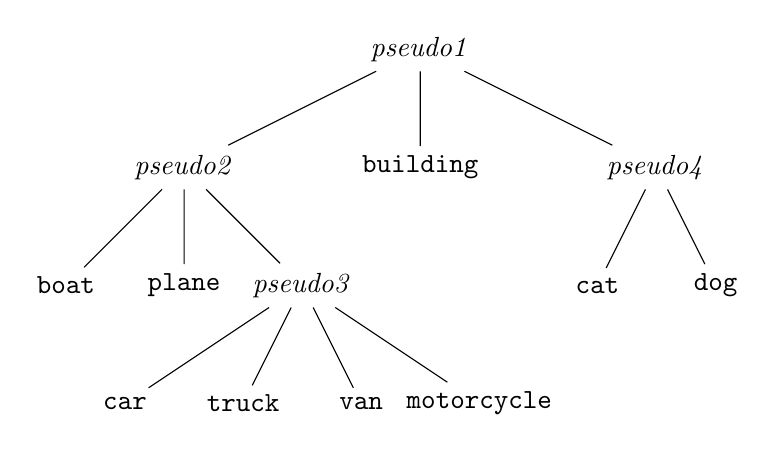
\begin{tikzpicture}
    [ level distance=1.5cm
    , level 1/.style={sibling distance=3cm}
    , level 2/.style={sibling distance=1.5cm}
    ]
\node {\textit{pseudo1}}
    child {node {\textit{pseudo2}}
      child {node {\texttt{boat}}}
      child {node {\texttt{plane}}}
      child {node {\textit{pseudo3}}
        child {node {\texttt{car}}}
        child {node {\texttt{truck}}}
        child {node {\texttt{van}}}
        child {node {\texttt{motorcycle}}}
      }
      }
    child {node {\texttt{building}}}
    child {node {\textit{pseudo4}}
      child {node {\texttt{cat}}}
      child {node {\texttt{dog}}}
    };
\end{tikzpicture}
\end{center}

We parameterize the weight vectors from the label tree as follows.
For each leaf node $i$ (equivalently for each class $i$),
we let the sequence $P_i$ denote the path from the leaf node to the root.
For example, using the label tree above,
we have
\begin{equation}
    P_{\texttt{truck}} = (\texttt{truck}, \textit{pseudo3}, \textit{pseudo2}, \textit{pseudo1} ) \qquad\text{and}\qquad
    P_{\texttt{cat}} = (\texttt{cat}, \textit{pseudo4}, \textit{pseudo1} )
    .
\end{equation}
Next, we associate a vector $\vv_i$ to each leaf and internal node $i$ in the tree structure.
In particular, there is a there is a vector $\vv_i$ for each class and for each pseudo-class.
Finally, we reparameterize the weights for the softmax cross entropy loss as the sum of the vectors along the paths.
Specifically, we set the weight vector for class $j$ to be 
\begin{equation}
    \label{eq:covertree-reparam}
    \w_j = \sum_{k\in P_j} \vv_k
    .
\end{equation}
Substituting \eqref{eq:covertree-reparam} into \eqref{eq:xentropy} gives us the final cover tree loss
\begin{equation}
    \ell(V;(\x,y)) = - \log \frac {\exp(-\sum_{k\in P_y}\trans\vv_k \x)}{\sum_{j=1}^c \exp(- \sum_{k\in P_j}\trans\vv_k \x)}
\end{equation}
where $V=(\vv_1,...,\vv_k)$,
and our goal is to minimize $\ell$ with respect to $V$.
Note that this loss can easily be computed in libraries like pytorch or tensorflow with the standard cross entropy loss functions.
The only change needed is to define the loss in terms of the sum of vectors $V$ instead of a variable tensor $W$.

\subsection{Analysis}

When analyzing stochastic gradient descent using the cross entropy loss,
it is common to assume that the parameter space is bounded.
Under the standard parameterization, we have that the weight vector for each class satisfies $\ltwo{\w_j} \le B$.
It immediately follows that $\lF{W} \le \sqrt{c}B$,
and from this and convergence results of SGD it follows that the generalization error is $O(\sqrt{k}B/n)$.
(See Theorem \ref{theorem:xentropy} above.)

The key idea of the tree loss is that we can reduce the bound on the size of the parameter space,
and this will result in the reduced sample complexity.
Let $\level k$ denote the level of node $k$ in the label tree.
Then we replace the constraints on the $\w_j$s with the following constraint on all $\vv_k$:
\begin{equation}
    \ltwo{\vv_k} \le \frac{B}{2^{\level k}}
    .
    \label{eq:tree-constraint}
\end{equation}
Notice that the original constraint \eqref{} immediately follows from the tree constraint \eqref{eq:tree-constraint} and the reparameterization \eqref{eq:covertree-reparam}.
One way to interpret this is that we have ``factored out'' our bounds on the $\w_i$ into bounds on the smaller $\vv_k$ components,
and because the $\vv_k$ vectors are shared between classes,
we can reduce the overall bound.
The following lemma bounds the Frobenius norm of the weight matrix $V$.

\begin{lemma}
    Assume that the label tree has at most $q$ nodes per level and $r$ levels.
    Then,
    \begin{equation}
        \lF{V} \le \tfrac12 Bq c^{(1 - 1/\log_2 q)}
    \end{equation}
    In particular, if $q=2$, then
    \begin{equation}
        \lF{V} \le B,
    \end{equation}
    which is independent of the number of classes $c$.
\end{lemma}
\begin{proof}
    We have the following chain of inequalities
    \begin{align}
        \lF{V} 
        &\le \sum_{k\in \text{nodes of the level tree}} \ltwo{\vv_k}
        \\
        &= \sum_{i=0}^r \sum_{k\in \text{nodes at level $i$}} \ltwo{\vv_k}
        \\
        &\le \sum_{i=0}^r B\left(\frac {q} {2}\right)^i
        \label{eq:lem:lFV:1}
        \\
        &=
        B\left(\frac{1 - (q/2)^{r+1}}{1-q/2}\right)
        \label{eq:lem:lFV:2}
        \\
        &\le
        B(q/2)^{r+1}.
        \label{eq:lem:lFV:3}
    \end{align}
    Line \eqref{eq:lem:lFV:1} follows from the fact that the number of nodes at level $i$ in the tree is upper bounded by $q^i$ and the the maximum L2 norm of a vector at level $i$ in the tree is $B/2^i$,so the sum of all vectors at level $i$ is bounded by $B(q/2)^i$.
    Lines \eqref{eq:lem:lFV:2} and \eqref{eq:lem:lFV:3} are standard properties of geometric series.

    Next, we show that
    \begin{equation}
        \left(\frac q 2\right)^r
        =
        \left(\frac q 2\right)^{\log_q n}
        =
        \frac{n}{2^{\log_q n}}
        =
        \frac{n}{2^{{\log_2 n}/{\log_2 q}}}
        =
        \frac{n}{n^{1/\log_2 q}}
        =
        n^{\left(1 - {1}/{\log_2 q}\right)}
        .
        \label{eq:lem:technical2}
    \end{equation}
    Substituting \eqref{eq:lem:technical2} into \eqref{eq:lem:lFV:3} gives the stated result.
\end{proof}

Substituting this Lemma into the SGD bounds gives us our main theorem: 

\begin{theorem}
\label{theorem:xentropy}
%Assume that for all $i\in[n]$, $\ltwo{x_i} \le \rho$,
    %and that for each class $i\in[c]$, $\ltwo{\w_i}\le B$.
\fixme{Add assumptions.}
Then the parameter vector $\bar W$ estimated from one epoch of SGD satisfies
\begin{equation}
    \E L_D(\bar W) - L_D(W^*) \le \frac {B\rho}{\sqrt n}
    ,
\end{equation}
which is independent of the number of classes $c$.
\end{theorem}
%Let $\mathcal L$ be a metric space over the set of labels,
%and $\ddim$ be the doubling dimension of $\mathcal L$.
%Then we build a ``cover tree'' from the class labels that respects the metric structure.
%This cover tree will have exactly $c$ leaf nodes, one for each class label,
%and $O(c)$ internal nodes.
%Why does this small change work?
%Intuitively, classes that have a small distance from each other should have similar weight vectors.

%\begin{lemma}
    %Under the conditions defined above, we have
%\begin{equation}
    %\label{eq:lFV-bound}
    %\lF{V} \le (\ddim \log c) B.
%\end{equation}
%\end{lemma}
%\begin{proof}
%\end{proof}

%Formally, we can bound the Frobenius norm of the weight matrix $V$ by
%which is significantly better than our bound on the weight matrix $W$ of only $\sqrt c B$.
%Substituting \eqref{eq:lFV-bound} into Theorem 14.12 of Shalev-Shwartz and Ben-David gives us that if SGD is run for $T$ iterations to compute parameter estimate $\bar W$,
%then
%\begin{equation}
    %\E L_D(\bar W) - L_D(W^*) \le \frac {\sqrt {\dim \mathcal L}B\rho\log c}{\sqrt T}
%\end{equation}
%where $W^* = \argmin L_D(W)$.


\subsection{Bias-variance tradeoff}
\label{sec:bias-var}

\section{Experiments}

\subsection{Synthetic data}

In this experiment we will demonstrate the cover tree loss's effectiveness on a simple multiclass logistic regression problem.
The problem will be specifically designed to be convex and have low intrinsic dimension in the class labels in order to illustrate the advantages of the cover tree loss.

Let $N$ be the standard normal distribution.
Then sample the matrices
\begin{align}
    U \sim N^{c\times a} \qquad\text{and}\qquad
    A \sim N^{a\times d},
\end{align}
and define the true parameter matrix to be
\begin{equation}
    W^* = UA.
\end{equation}
For all $i \in [c]$, the row $\w_i^*$ of $W^*$ corresponds to the parameter vector for class $i$ and has dimension $d$.
The variable $a$ controls the intrinsic dimensionality of the problem.
When $a$ is small, then many class labels will be similar to each other;
but as $a$ increases, the class labels will have increasingly less structure.
When $a$ is known in advance, then we can use weight matrix factorization and set $e=a$.

For each data point $i\in[n]$,
we sample the data point according to the following rules:
\begin{align}
    y_i &\sim \text{Uniform}([c]), \text{and} \\
    \x_{i} &\sim \mathcal N(\w^*_{y_i}; \sigma),
\end{align}
where $\sigma$ controls the noise in the dataset.
Increasing $\sigma$ adds noise and makes classes harder to distinguish,
whereas decreasing $\sigma$ reduces noise and makes the classes easier to distinguish.

With our problem defined in this way, it is clear that
\begin{equation}
    \argmin_{W} \tfrac 1 n \ell(W; \x_i, y_i)
\end{equation}
converges to $W^*$ using the standard cross entropy loss and both the matrix factorization and cover tree reparameterizations.
\fixme{You should prove this for yourself.}
Figure \ref{fig:synthetic-results} shows that the cover tree loss converges at a faster rate.

\begin{figure}[h]
    \centering
    \includegraphics[width=0.3\textwidth]{example-image-a}
    \includegraphics[width=0.3\textwidth]{example-image-b}
    \includegraphics[width=0.3\textwidth]{example-image-c}
    \caption{
        \fixme{We need a plot of loss vs number of data points ($n$), vs dimension ($d$), and vs randomness ($sigma$). These plots should all be log-log plots.  For each of these experiments, you should write to shell scripts: the first to generate the data and the second to plot the data.  These shell scripts should be easy to run in order to easily replicate your experiments.}}
    \label{fig:synthetic-results}
\end{figure}

\subsubsection{Alternative synthetic experiments}

In multilabel classification, it is common for the classes to be unbalanced.
We would like to show that the cover tree loss works well for unbalanced data.
A good way to do that is to change the distribution that $y_i$ is drawn from,
and a geometric distribution is a likely good alternative.

The covertree loss can work well even when the weight matrix has non-linear intrinsic structure.
We should adapt the $\w*_i$ vectors to sit on a manifold instead of a hyperplane to demonstrate this fact.

\subsection{Pseudo-synthetic data}
In a pseudo-synthetic dataset, we take a non-synthetic dataset and modify it.
\fixme{describe your procedure for generating pseudo-synthetic data and all the experiments that you plan to run}

\begin{table}[h]
    \centering
    \begin{tabular}{llrrr}
    \toprule
    Dataset  & type & data points ($n$) & dimensions ($d$) & classes ($c$) \\
    \midrule
    MNIST    & image & 60,000 & - & 10\\
    CIFAR10  & image & 60,000 & - & 10 \\
    CIFAR100 & image & 60,000 & - & 100 \\
    IMAGENET & image & 1,281,167 & - & 1,000\\
     & text & - & - & - \\
    \bottomrule
\end{tabular}
\caption{
    \fixme{complete this table with the datasets you plan to use.}
}


\end{table}

\subsection{Real world twitter data}
\fixme{Write a description of the experiment.}

%%%%%%%%%%%%%%%%%%%%%%%%%%%%%%%%%%%%%%%%%%%%%%%%%%%%%%%%%%%%%%%%%%%%%%%%%%%%%%%%
\bibliographystyle{plainnat}
\bibliography{paper}

\end{document}


